\section{Całki podwójne}

Zapis: $ \iint\limits_{D} f(x,y)\, dxdy $, gdzie zbiór $D$ i funkcja $f$ są odpowiednio regularne.

Definicja może być skonstruowana poprzez:
\begin{itemize}
    \item $n$ -- tą sumę całkową (sumę Riemanna) -- podobnie jak w AM1
    \item tzw. \underline{całki iterowane}
\end{itemize}
\bigskip

Przypadek podstawowy -- $D$ jest prostokątem
\[ D = [a,b] \times [c,d] = \{ (x,y): a \leq x \leq b, \ c \leq y \leq d \} \]
\medskip

\begin{tw}{Całka w sensie Riemanna}

Dzielimy $D$ na $n$ prostokątów o bokach poziomych o długości $\Delta X$ i bokach pionowych o długości $\Delta y_i, \ i = 1,2,...,n$.
W każdym z prostokątów wybieramy dowolny punkt $P_i = (a_i, b_i)$.

Sumą Riemanna ($n$ -- tą sumę całkową) funkcji $f$ na $D$ jest
\[ S_n = \sum\limits_{n=1}^{n} \Delta x_i \cdot \Delta y_i \cdot f(a_i, b_i) \]
\end{tw}

\begin{center}
    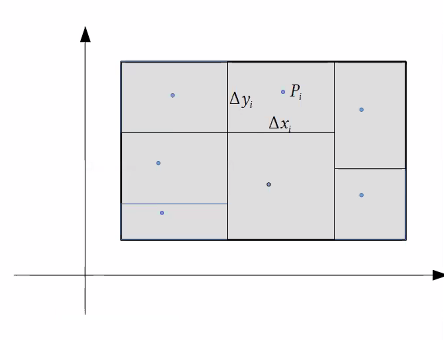
\includegraphics[scale=0.8]{img/prostokat1.png}
\end{center}

Jeżeli dla $ n \to \infty, \ \Delta x_i \to 0, \ \Delta y_i \to 0 $ \ granica \ $ \lim_{n \to \infty} S_n $ \ istnieje i \underline{nie zależy}
od wyboru prostokątów oraz punktów $P_i$ to nazywamy ją całką podwójną z $f$ na prostokącie $D$ i oznaczamy przez \ $ \iint\limits_D f(x,y) \, dxdy $.
\bigskip

\begin{tw}{Twierdzenie}

Gdy $f$ jest ciągła na prostokącie $D$ to całka podwójna z $f$ na $D$ istnieje.
\bigskip

Interpretacja geometryczna dla $ f \geq 0 $ na $D$: $S_n$ to suma objętości prostopadłościanów o krawędziach $ \Delta x_i, \ \Delta y_i $ oraz $ f(a_i, b_i) $.
Prostopadłościany te przybliżają bryłę o podstawie $D$, ścianach pionowych i ograniczonej z góry przez powierzchnię $f$.
\end{tw}


Granica $S_n$ daje objętość tej bryły.

\begin{center}
    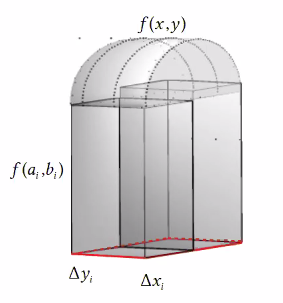
\includegraphics[scale=0.5]{img/prostowalec.png}
\end{center}

Dla $ D = [a,b] \times [c,d] $ są to całki postaci

\[ \int\limits_c^d dy \int\limits_{a}^{b} f(x,y) \, dx = \int\limits_{c}^{d} dy \left( \int\limits_{a}^{b} f(x,y) \, dx \right) \]
\begin{center}oraz \end{center}
\[ \int\limits_a^b dx \int\limits_{c}^{d} f(x,y) \, dy = \int\limits_{a}^{b} dx \left( \int\limits_{c}^{d} f(x,y) \, dy \right) \]

\begin{tw}{Twierdzenie}

Gdy $f$ jest ciągła na $D$ to
\[ \int\limits_{c}^{d} dy \int\limits_{a}^{b} f(x,y) \, dx = \int\limits_{a}^{b} dx \int\limits_{c}^{d} f(x,y) \, dy = \iint\limits_D f(x,y) \, dxdy \]

\end{tw}

\textbf{Przykład}

\[ D = [0,1] \times [-1,1], \ f(x,y) = 2x + 3y^2 \]

\[ \int\limits_{0}^{1} dx \int\limits_{-1}^{1} (2x+3y^2) \, dy = \int\limits_{0}^{1} dx \left[ 2xy + y^3 \right]_{y = -1}^{y=1} 
= \int\limits_{0}^{1} dx (4x+2) = \left[ 2x^2 + 2x \right]_0^1 = 4 - 0 = 4 \]

\begin{center} W odwrotnej kolejności \end{center}
\[ \int\limits_{-1}^{1} dy \int\limits_{0}^{1} (2x+3y^2)\, dx = \int\limits_{-1}^{1} dy \left[ x^2 + 3y^2x \right]_{x=0}^{x=1} 
= \int\limits_{-1}^{1} dy (3y^2 + 1) = \left[ y^3 + y \right]_{-1}^{1} = 2- (-2) = 4 \]

Przypadek ogólny -- całki po tzw. \underline{obszarach normalnych}.

Są to zbiory postaci:
\[ D = \{ (x,y): a \leq x \leq b, \ d(x) \leq y \leq g(x) \} \quad \textrm{lub} \quad D = \{ (x,y): a \leq y \leq b, \ d(y) \leq x \leq g(y) \} \]

Ponadto funkcje $d$ i $g$ są ciągłe.
\bigskip

Definicja całki podwójnej w sensie Riemanna jest analogiczna jak dla prostokąta.

\[ \int\limits_{a}^{b} dx \int\limits_{d(x)}^{g(x)} f(x,y)\, dy = \int\limits_{a}^{b} dx \left( \ \int\limits_{d(x)}^{g(x)} f(x,y)\, dy \right) \]
\begin{center} lub \end{center}
\[ \int\limits_{c}^{d} dy \int\limits_{d(x)}^{g(x)} f(x,y)\, dx = \int\limits_{a}^{b} dy \left( \ \int\limits_{d(x)}^{g(x)} f(x,y)\, dx \right) \]

\begin{tw}{Twierdzenie}

Gdy $f$ jest ciągła na obszarze normalnym to całka podwójna $ \iint\limits_{D} f(x,y)\, dxdy $ istnieje i jest równa każdej z całek iterowanych. 

\end{tw}

\textbf{Przykład}

$ f(x,y) = xy $

$D$ jest ograniczony krzywymi $ x=0, \ x=2, y=e^x $
\medskip

\begin{center}
    Rysunek obszaru:
    
    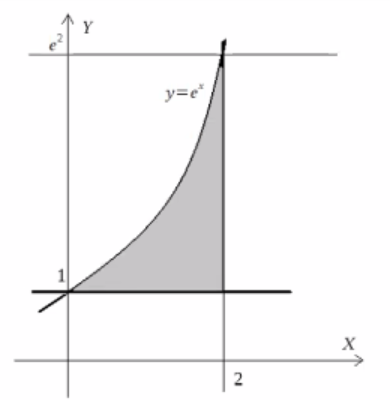
\includegraphics[scale=0.7]{img/krzywetrojkat.png}
\end{center}

Mamy \ $ D: 0 \leq x \leq 2, \ 1 \leq y \leq e^x $. Czyli całka jest równa
\[ \int\limits_{0}^{2} dx \int\limits_{1}^{e^x} xy \, dy = \int\limits_{0}^{2} dx \left[ \frac{xy^2}{2} \right]_{1}^{e^x} 
= \int\limits_{0}^{2} dx \left( \frac{xe^{2x}}{2} - \frac{x}{2} \right) = \frac{1}{2} \int\limits_{0}^{2} xe^{2x}\, dx - \frac{1}{2} \int\limits_{0}^{2} x\, dx \]

Ta druga całka wynosi 2.

Tą pierwszą liczymy przez części:
\[ \int xe^{2x} = \frac{1}{2} xe^{2x} - \int 1 \cdot \frac{1}{2} e^{2x} \, dx = \frac{1}{2} xe^{2x} - \frac{1}{4} e^{2x} + C \]
\[ \begin{vmatrix}
    f(x) = x & g'(x) = e^{2x} \\
    f'(x) = 1 & g(x) = \frac{1}{2}e^{2x} 
\end{vmatrix} \]

Zatem
\[ \int\limits_{0}^{2} xe^{2x} \, dx = e^4 - \frac{1}{4}e^4 + \frac{1}{4} = \frac{3}{4}e^4 + \frac{1}{4} \]

Całość:
\[ \iint\limits_D f(x,y) \, dxdy = \frac{1}{2} \left( \frac{3}{4}e^4 + \frac{1}{4} \right) - \frac{1}{2} \cdot 2 = \frac{3}{8}e^4 - \frac{7}{8} \]
\bigskip

\begin{tw}{Własności całki podwójnej}
\begin{itemize}
    \item $ \iint\limits_D \left( f(x,y) \pm g(x,y) \right)\, dxdy = \iint\limits_D f(x,y)\, dxdy \pm \iint\limits_D g(x,y)\, dxdy $
    \item $ \iint\limits_D c \cdot f(x,y)\, dxdy = c \iint\limits_D f(x,y)\, dxdy $
    \item gdy \ $ D = D_1 \cup D_2 $ \ i \ $ D_1, D_2 $ \ są rozłączne to
    $ \iint\limits_D f(x,y)\, dxdy = \iint\limits_{D_1} f(x,y)\, dxdy + \iint\limits_{D_2} f(x,y)\, dxdy $
\end{itemize}
\end{tw}